\chapter{Experiments and Results}
\label{ch:results}

This chapter describes the benchmarks and the evaluation protocol, and presents the results: accuracy on each benchmark, latency and routing, the effect of the LLM arbiter, the empirical behaviour of the conformal layer, the calibration of the NLI probabilities, the hypothesis tests that compare these results, and an analysis of the errors.

\section{Benchmarks}

\paragraph{FEVER}~\citep{thorne2018fever}. Claims written by annotators who altered sentences from Wikipedia, labelled \textsc{Supports}, \textsc{Refutes} or \textsc{Not Enough Info}. The detector is evaluated on the \textsc{Supports} and \textsc{Refutes} claims of the validation split. FEVER tests entity retrieval and NLI on encyclopedic facts that do not change over time, and is the primary benchmark.

\paragraph{FreshQA}~\citep{vu2023freshllms}. Questions whose answers may change over time, plus false-premise questions, with answers maintained by the authors. Because the detector verifies claims rather than answering questions, each question--answer pair is converted once into a declarative claim by an LLM: a normal question and its answer (\emph{``Who is the CEO of Google?''} -- \emph{``Sundar Pichai''}) become a true claim (\emph{``Sundar Pichai is the CEO of Google''}); a false-premise question (\emph{``When was League of Legends 2 released?''}) becomes its false premise as a claim (\emph{``League of Legends 2 was released''}). Gold answers are dated snapshots, so only \emph{never-changing} and \emph{slow-changing} questions are used. FreshQA tests web retrieval, temporal reasoning and false-premise detection.

Benchmarks built from synthetic perturbations of a fixed reference text are not used: their ``false'' claims are often true in the open world that this detector searches, which would penalise correct verdicts.

\section{Evaluation Protocol}

\begin{enumerate}[itemsep=0.2em]
  \item \textbf{Stratified sampling.} Each benchmark is split into 15 non-overlapping sets of 20 claims (10 true, 10 false), drawn with a fixed random seed, giving 300 claims per benchmark and 600 in total. FreshQA has only 147 never- and slow-changing false claims, so its fifteenth set holds the last 7 false and 13 true claims.
  \item \textbf{Verification.} Each claim is verified end to end with live Wikipedia, web and LLM calls, using the single configuration described in Chapter~\ref{ch:method}. FreshQA claims also receive the original question as context.
  \item \textbf{Scoring.} The prediction is compared with the gold label. \Unk{} counts as wrong, and on a false claim as a missed hallucination. A claim whose verification hits an LLM infrastructure failure is retried rather than scored, so outages are never counted as abstentions.
\end{enumerate}

\paragraph{Metrics.} The positive class is a hallucination (gold label \textsc{Refutes}). A false claim flagged \Con{} is a true positive (TP); a true claim flagged \Con{} a false positive (FP, a false accusation); a false claim judged \Sup{} or \Unk{} a false negative (FN, a missed hallucination); a true claim judged \Sup{} a true negative (TN). A true claim left \Unk{} is counted only as an accuracy error. Then
\begin{equation}
  \text{Precision} = \frac{TP}{TP + FP}, \qquad \text{Recall} = \frac{TP}{TP + FN}, \qquad F_1 = \frac{2\,TP}{2\,TP + FP + FN}.
\end{equation}

\section{Main Results}

Table~\ref{tab:main} summarises the pooled results. For FEVER, 134 false claims were flagged \Con, 15 judged \Sup{} and 1 left \Unk; 138 true claims were judged \Sup, 9 flagged \Con{} and 3 left \Unk. Hence accuracy $= (134 + 138)/300 = 90.7\%$, precision $= 134/143 = 0.94$, recall $= 134/150 = 0.89$ and $F_1 = 268/293 = 0.91$.

\begin{table}[htbp]
\centering
\caption{Pooled results over 300 claims per benchmark (fifteen sets of 20).}
\label{tab:main}
\resizebox{\textwidth}{!}{%
\begin{tabular}{@{}lcccccccc@{}}
\toprule
Benchmark & Accuracy & Wilson 95\% CI & Precision & Recall & $F_1$ & TP/FP/FN/TN & \Unk & Latency \\
\midrule
FEVER & 90.7\% & [86.8\%, 93.5\%] & 0.94 & 0.89 & 0.91 & 134/9/16/138 & 4 & 8.5\,s \\
FreshQA & 82.3\% & [77.6\%, 86.2\%] & 0.91 & 0.80 & 0.85 & 117/12/30/130 & 15 & 11.3\,s \\
\bottomrule
\end{tabular}}
\end{table}

\begin{figure}[htbp]
\centering
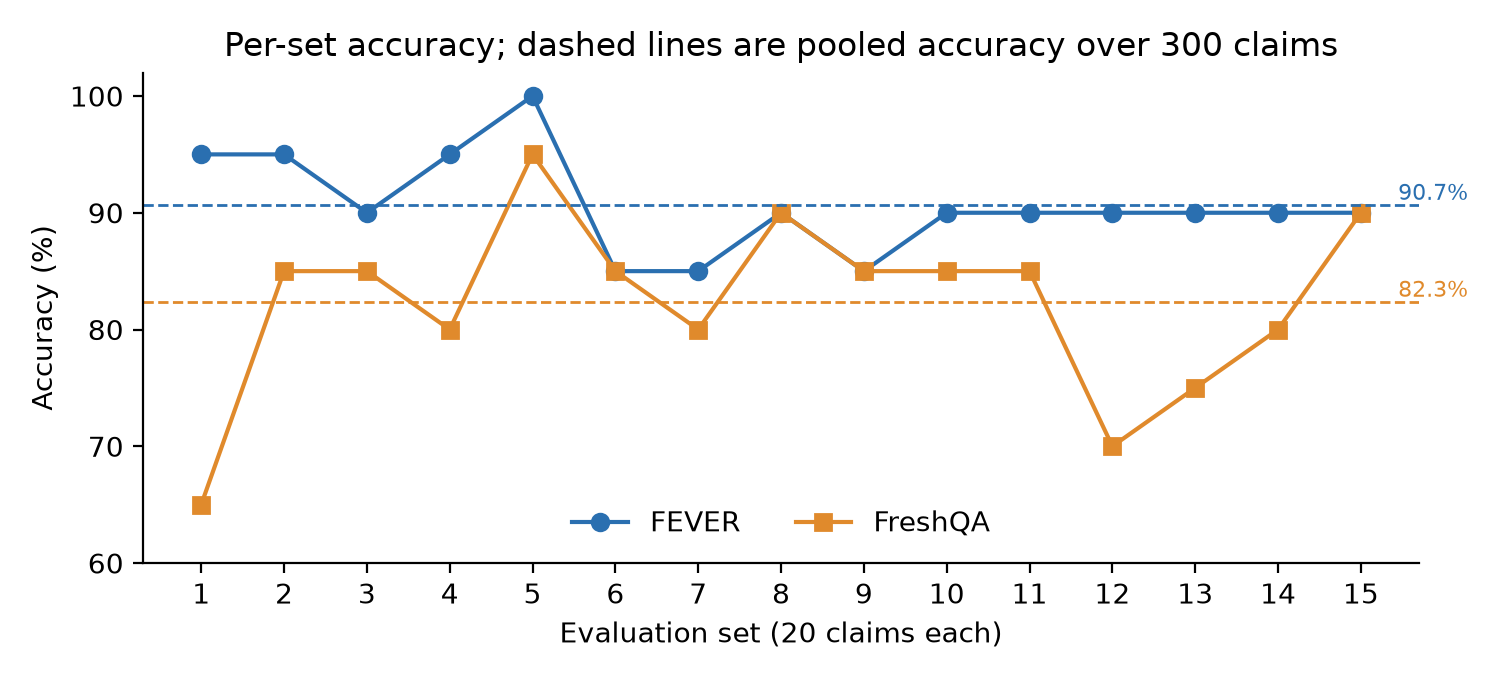
\includegraphics[width=0.95\textwidth]{per_set_accuracy.png}
\caption{Accuracy on each of the fifteen sets of 20 claims. With 20 claims per set, one error moves the accuracy by 5 points; the pooled figures are the ones to quote.}
\label{fig:perset}
\end{figure}

\begin{table}[htbp]
\centering
\caption{Per-set results (correct verdicts out of 20).}
\label{tab:perset}
\small
\begin{tabular}{@{}l*{15}{c}c@{}}
\toprule
Set & 1 & 2 & 3 & 4 & 5 & 6 & 7 & 8 & 9 & 10 & 11 & 12 & 13 & 14 & 15 & Total \\
\midrule
FEVER   & 19 & 19 & 18 & 19 & 20 & 17 & 17 & 18 & 17 & 18 & 18 & 18 & 18 & 18 & 18 & 272 \\
FreshQA & 13 & 17 & 17 & 16 & 19 & 17 & 16 & 18 & 17 & 17 & 17 & 14 & 15 & 16 & 18 & 247 \\
\bottomrule
\end{tabular}
\end{table}

\paragraph{Intervals for precision, recall and $F_1$.} Table~\ref{tab:prf} gives the 95\% intervals of the hallucination-class metrics (Section~\ref{sec:prf-intervals}): Wilson intervals for precision and recall, and percentile-bootstrap intervals for $F_1$ (10{,}000 resamples). Even the lower ends of the precision intervals are above 0.84 (0.885 for FEVER, 0.844 for FreshQA, 0.885 pooled), so false accusations are rare with high confidence; the recall intervals of the two benchmarks barely overlap, which locates the gap between them in missed hallucinations.

\begin{table}[H]
\centering
\caption{Precision, recall and $F_1$ of the hallucination class with 95\% intervals.}
\label{tab:prf}
\begin{tabular}{@{}lccc@{}}
\toprule
Benchmark & Precision (Wilson) & Recall (Wilson) & $F_1$ (bootstrap) \\
\midrule
FEVER & 0.937 [0.885, 0.967] & 0.893 [0.834, 0.933] & 0.915 [0.879, 0.945] \\
FreshQA & 0.907 [0.844, 0.946] & 0.796 [0.724, 0.853] & 0.848 [0.801, 0.890] \\
Pooled & 0.923 [0.885, 0.949] & 0.845 [0.800, 0.882] & 0.882 [0.853, 0.910] \\
\bottomrule
\end{tabular}
\end{table}

\paragraph{Consistency of the runs.} The fifteen sets were evaluated in three runs of five sets each. FEVER scored 95, 87 and 90 of 100 in the three runs: the chi-square test of equal accuracy gives $X^2 = 3.86$ with 2 degrees of freedom, $p = e^{-1.93} = 0.15$. FreshQA scored 82, 85 and 80 ($X^2 = 0.87$, $p = 0.65$). In both cases the runs are consistent with one underlying accuracy.

\paragraph{FEVER versus FreshQA.} FreshQA is significantly harder. The difference in accuracy is 8.3 points (Newcombe 95\% interval [2.9, 13.8] points); the two-proportion $z$-test gives $z = 2.99$, $p = 0.003$, and Fisher's exact test $p = 0.004$. Precision is similar (0.94 against 0.91); the gap lies in recall (0.89 against 0.80) and in abstentions (4 against 15). FreshQA's false premises and claims about the present are more often accepted by the NLI model or left \Unk{} when the evidence does not settle them, and some of its gold answers are contradicted by current evidence (Section~\ref{sec:errors}).

\section{Latency, Routing and Cost}
\label{sec:routing-results}

Table~\ref{tab:latency} gives the latency and the number of LLM calls per claim. Latency was measured end to end, with live Wikipedia, web and Gemini calls, on an Apple M1 laptop. Light LLM calls (query generation and rewriting) took 1.3\,s on average and heavy calls (arbitration, absence evaluation) 2.9\,s.

\begin{table}[H]
\centering
\caption{Latency and LLM usage per claim.}
\label{tab:latency}
\begin{tabular}{@{}lcccc@{}}
\toprule
Benchmark & Mean latency & Median & 90th percentile & LLM calls per claim \\
\midrule
FEVER & 8.5\,s & 8.0\,s & 12.1\,s & 1.05 \\
FreshQA & 11.3\,s & 9.9\,s & 19.5\,s & 1.45 \\
\bottomrule
\end{tabular}
\end{table}

Table~\ref{tab:routes} and Figure~\ref{fig:routing} show how the claims were routed and how accurate each route was. The conformal layer kept 413 of the 600 claims on the fast path, and these were correct 89\% of the time (368 of 413); the 187 claims it passed on, which are the harder ones, were correct 81\% of the time after LLM review (151 of 187).

\begin{table}[H]
\centering
\caption{Claims and accuracy by route.}
\label{tab:routes}
\begin{tabular}{@{}lccc@{}}
\toprule
Benchmark & NLI verdict stands & Lightweight review & Full escalation \\
\midrule
FEVER   & 212 / 229 (93\%) & 30 / 35 (86\%) & 30 / 36 (83\%) \\
FreshQA & 156 / 184 (85\%) & 47 / 54 (87\%) & 44 / 62 (71\%) \\
\bottomrule
\end{tabular}
\end{table}

\begin{figure}[htbp]
\centering
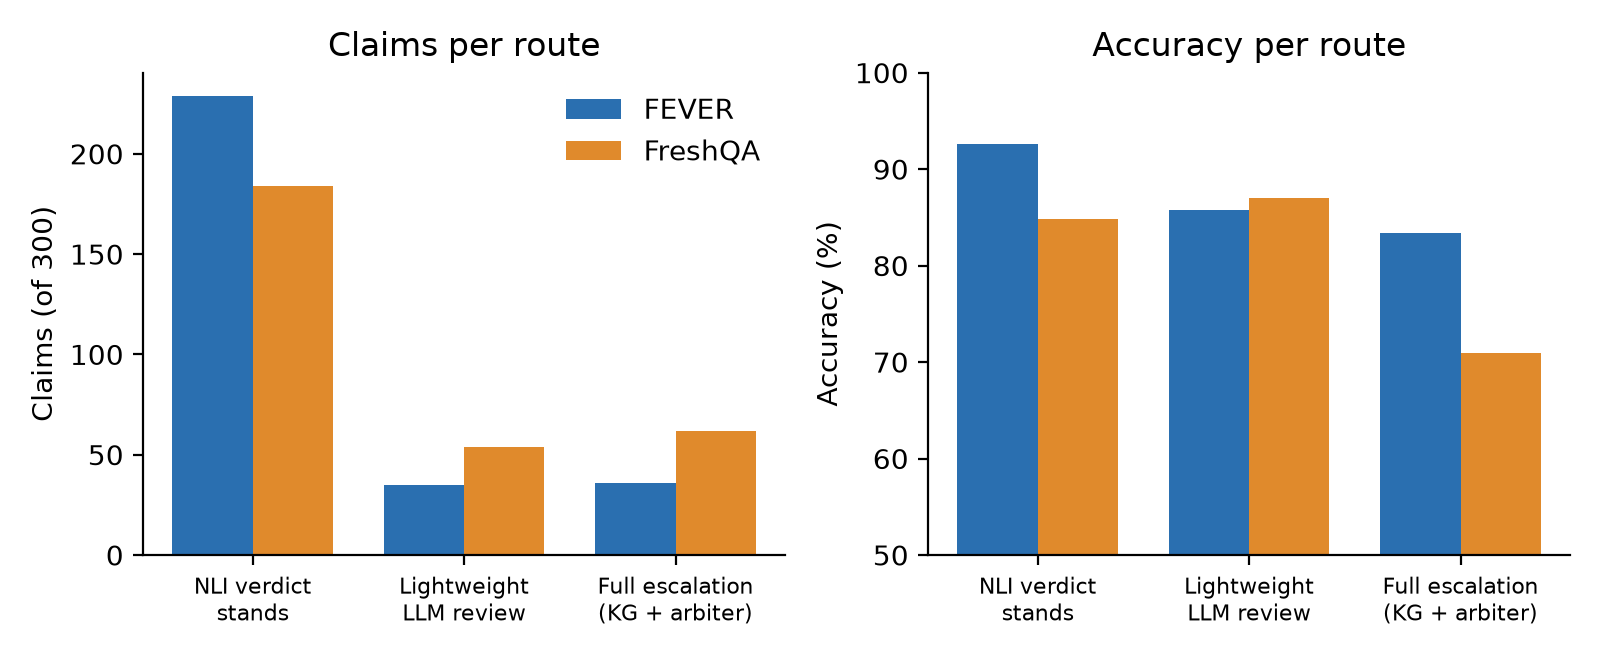
\includegraphics[width=0.95\textwidth]{routing.png}
\caption{Number of claims and accuracy for each route of the cascade.}
\label{fig:routing}
\end{figure}

LLM calls averaged 0.86 per claim when the NLI verdict stood (mostly query generation), 1.88 with a lightweight review and 2.32 with full escalation. Fully escalated claims, which add the Wikidata evidence and arbitration, account for the long tail of the latency distribution.


\section{Effect of the LLM Arbiter}

The computation trace records the NLI verdict just before arbitration, so the arbiter's effect can be measured on every claim it decided (Table~\ref{tab:arbiter}, Figure~\ref{fig:arbiter}).

\begin{table}[htbp]
\centering
\caption{LLM arbiter against the NLI verdict it replaced.}
\label{tab:arbiter}
\begin{tabular}{@{}lccccc@{}}
\toprule
Benchmark & Claims decided & Fixed & Broken & Both right & Both wrong \\
\midrule
FEVER & 71 & 18 & 7 & 42 & 4 \\
FreshQA & 116 & 42 & 8 & 49 & 17 \\
\textbf{Total} & \textbf{187} & \textbf{60} & \textbf{15} & \textbf{91} & \textbf{21} \\
\bottomrule
\end{tabular}
\end{table}

\begin{figure}[htbp]
\centering
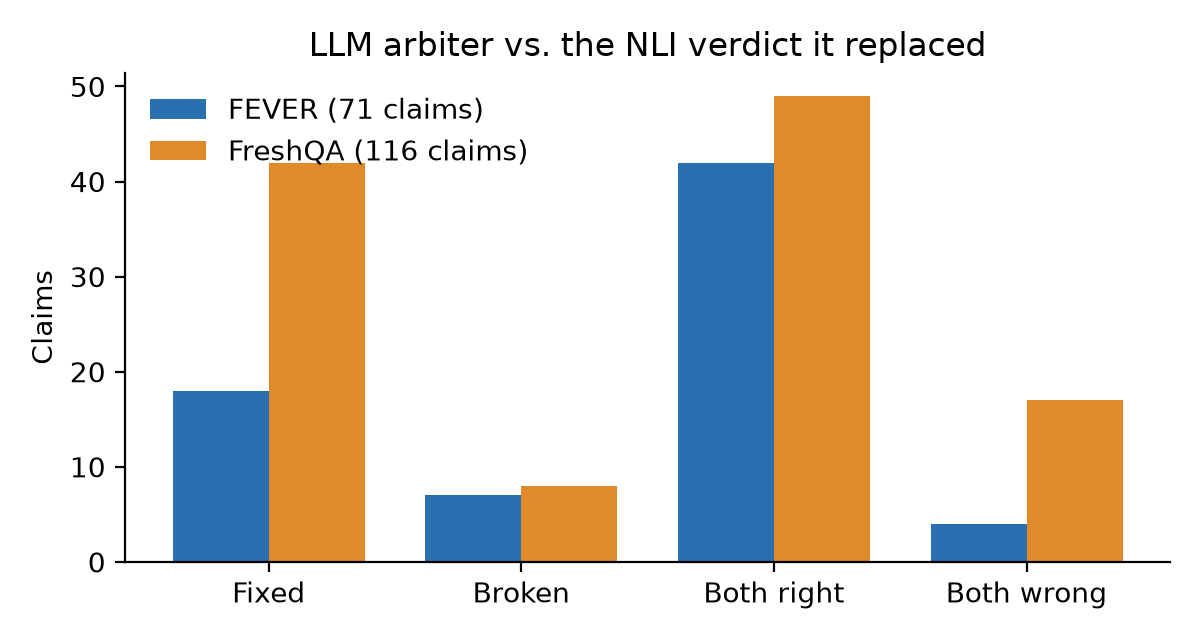
\includegraphics[width=0.72\textwidth]{arbiter_effect.png}
\caption{Claims decided by the LLM arbiter, by whether the NLI verdict and the final verdict were right.}
\label{fig:arbiter}
\end{figure}

The arbiter corrected 60 verdicts and spoiled 15. By the exact McNemar test~\eqref{eq:mcnemar}, $p = 1.6 \times 10^{-7}$: the improvement is highly significant. Per benchmark, FreshQA gives 42 against 8 ($p = 1.2 \times 10^{-6}$) and FEVER 18 against 7 ($p = 0.043$), the latter significant on its own but not after correction for multiple testing (Section~\ref{sec:test-summary}).

\section{Ablation Study}
\label{sec:ablation}

To show what each stage of the cascade contributes, the verdict every claim would have received with that stage removed was reconstructed from its computation trace. The trace records the NLI verdict the scoring rule gave before any LLM review, so removing an LLM stage simply replaces the final verdict of the claims that stage decided by that NLI verdict. The reconstruction is therefore exact and needs no new model run or LLM call. Five variants are compared with the full pipeline:
\begin{itemize}[itemsep=0.2em]
  \item \textbf{Always \Sup}: the trivial detector that never flags a hallucination, as a floor.
  \item \textbf{NLI only, first pass}: the first NLI verdict, with no query rewrite and no LLM verdict. The only LLM calls left are those of query generation for claims outside its fast path.
  \item \textbf{NLI only}: the NLI verdict after the query rewrite, with no LLM verdict.
  \item \textbf{No lightweight review}: lone and contested contradictions are accepted without review (the original ``highest confidence wins'' rule); escalation is kept.
  \item \textbf{No full escalation}: escalated claims keep their NLI verdict (no Wikidata evidence, no arbitration); lightweight reviews are kept.
\end{itemize}
Each variant is compared with the full pipeline by the exact McNemar test on the same claims. The five pooled comparisons form their own family and are Holm-corrected within it; this family is separate from the eight tests of Section~\ref{sec:test-summary}, whose adjusted $p$-values are unchanged.

\begin{table}[H]
\centering
\caption{Ablation study. Accuracy per benchmark and pooled (600 claims), with pooled $F_1$, mean LLM calls per claim, and the exact McNemar test against the full pipeline ($b$: claims right only with the full pipeline; $c$: right only with the variant).}
\label{tab:ablation}
\resizebox{\textwidth}{!}{%
\begin{tabular}{@{}lccccccc@{}}
\toprule
Variant & FEVER & FreshQA & Pooled (Wilson 95\% CI) & Pooled $F_1$ & LLM calls & $b$ / $c$ & $p$ (Holm) \\
\midrule
Always \Sup & 50.0\% & 51.0\% & 50.5\% [46.5, 54.5] & 0.00 & 0.00 & 251 / 35 & $9.7 \times 10^{-41}$ \\
NLI only, first pass & 85.7\% & 62.7\% & 74.2\% [70.5, 77.5] & 0.83 & 0.80 & 88 / 14 & $1.1 \times 10^{-13}$ \\
NLI only & 87.0\% & 71.0\% & 79.0\% [75.6, 82.1] & 0.83 & 0.94 & 60 / 15 & $4.8 \times 10^{-7}$ \\
No lightweight review & 90.3\% & 77.0\% & 83.7\% [80.5, 86.4] & 0.86 & 1.10 & 22 / 5 & $0.0015$ \\
No full escalation & 87.3\% & 76.3\% & 81.8\% [78.5, 84.7] & 0.86 & 1.08 & 38 / 10 & $1.2 \times 10^{-4}$ \\
\textbf{Full pipeline} & \textbf{90.7\%} & \textbf{82.3\%} & \textbf{86.5\% [83.5, 89.0]} & \textbf{0.88} & \textbf{1.25} & -- & -- \\
\bottomrule
\end{tabular}}
\end{table}

\begin{figure}[H]
\centering
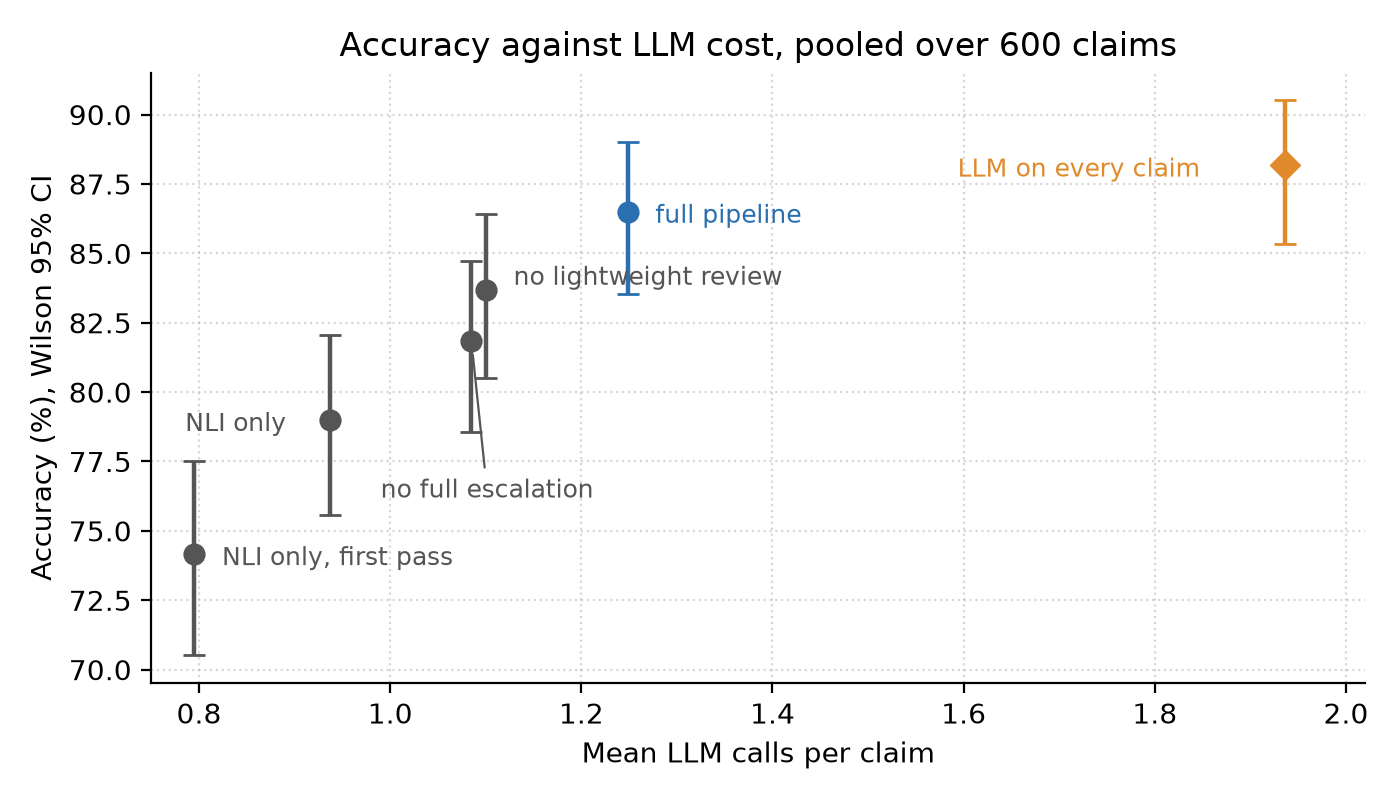
\includegraphics[width=0.8\textwidth]{ablation_cost.png}
\caption{Pooled accuracy of each ablation, and of the LLM-only baseline of Section~\ref{sec:llm-baseline}, against the mean number of LLM calls per claim. ``NLI only'' includes the query rewrite.}
\label{fig:ablation}
\end{figure}

Every stage contributes, and every pooled difference survives the Holm correction (Table~\ref{tab:ablation}, Figure~\ref{fig:ablation}):
\begin{itemize}[itemsep=0.3em]
  \item \textbf{The LLM stages as a whole} raise pooled accuracy from 79.0\% to 86.5\% for 0.31 extra LLM calls per claim, because they are spent only on the claims the conformal layer and the corroboration rule flag.
  \item \textbf{The query rewrite} lifts the NLI verdict from 74.2\% to 79.0\% pooled, almost entirely on FreshQA (62.7\% to 71.0\%), and halves the claims left \Unk{} (85 to 40) for 0.14 extra calls per claim.
  \item \textbf{The lightweight review} matters mostly for \emph{precision}, the property the design protects (Section~\ref{ch:formulation}): without it, precision falls from 0.92 to 0.85 pooled and from 0.91 to 0.79 on FreshQA, because lone and contested NLI contradictions are accepted as false accusations. On FEVER alone the review changes only 7 verdicts (4 against 3) and its effect is not measurable.
  \item \textbf{Full escalation} adds 4.7 points pooled (38 claims fixed, 10 broken) and cuts abstentions from 44 to 19.
\end{itemize}
The two LLM stages are complementary: removing either costs a significant amount of accuracy, and they act on different claims.

\section{Comparison with an LLM-Only Baseline}
\label{sec:llm-baseline}

The ablation removes stages from the cascade. The opposite question is whether the cascade is needed at all: why not let the LLM arbiter decide every claim? To answer it, every claim received one arbitration call on its retrieved evidence, with the same prompt and settings as the live pipeline (dialectical mode, strict premises, the claim's domain). On the 187 claims the LLM already decided in the benchmark run, the two systems are identical by construction, so they can differ only on the 413 claims the NLI verdict settled. Of these, 225 already had an LLM review of the same evidence from the earlier analyses (Sections~\ref{sec:coverage-retrieved} and~\ref{sec:crossfit-results}). The remaining 188 were arbitrated for this comparison (187 calls, since one FEVER claim appears twice), all answered by \code{gemini-3.5-flash-lite}, the model of the benchmark run.

\begin{table}[H]
\centering
\caption{The cascade against an LLM verdict for every claim. The baseline's latency is estimated by adding the mean measured arbitration time (3.0\,s) to every claim the NLI verdict settled.}
\label{tab:llm-baseline}
\resizebox{\textwidth}{!}{%
\begin{tabular}{@{}llcccccc@{}}
\toprule
Benchmark & System & Accuracy (Wilson 95\% CI) & Precision & Recall & $F_1$ & LLM calls per claim & Mean latency \\
\midrule
FEVER & Cascade & 90.7\% [86.8, 93.5] & 0.94 & 0.89 & 0.91 & 1.05 & 8.5\,s \\
 & LLM on every claim & 91.3\% [87.6, 94.0] & 0.94 & 0.91 & 0.93 & 1.81 & 10.8\,s \\
\midrule
FreshQA & Cascade & 82.3\% [77.6, 86.2] & 0.91 & 0.80 & 0.85 & 1.45 & 11.3\,s \\
 & LLM on every claim & 85.0\% [80.5, 88.6] & 0.90 & 0.87 & 0.88 & 2.06 & 13.2\,s \\
\midrule
Pooled & Cascade & 86.5\% [83.5, 89.0] & 0.92 & 0.85 & 0.88 & 1.25 & 9.9\,s \\
 & LLM on every claim & 88.2\% [85.3, 90.5] & 0.92 & 0.89 & 0.91 & 1.94 & 12.0\,s \\
\bottomrule
\end{tabular}}
\end{table}

The paired comparison (Table~\ref{tab:llm-baseline-paired}) uses the exact McNemar test (Section~\ref{sec:tests}). With $b$ claims right only under the cascade and $c$ right only under the baseline, the difference in accuracy and its paired standard error are
\[
  \hat{d} = \frac{c - b}{N}, \qquad \widehat{\mathrm{SE}}(\hat{d}) = \frac{1}{N} \sqrt{b + c - \frac{(c - b)^2}{N}} .
\]
The last column is the number of claims McNemar's test would need for 80\% power against a difference of the observed size (Section~\ref{sec:power}).

\begin{table}[H]
\centering
\caption{Paired comparison of the LLM-only baseline with the cascade.}
\label{tab:llm-baseline-paired}
\resizebox{\textwidth}{!}{%
\begin{tabular}{@{}lccccc@{}}
\toprule
Benchmark & Cascade right only & Baseline right only & $p$ & Difference (95\% CI) & Claims for 80\% power \\
\midrule
FEVER & 7 & 9 & 0.80 & $+0.7$ [$-1.9$, $+3.3$] points & 9{,}417 \\
FreshQA & 11 & 19 & 0.20 & $+2.7$ [$-0.9$, $+6.2$] points & 1{,}102 \\
Pooled & 18 & 28 & 0.18 & $+1.7$ [$-0.5$, $+3.9$] points & 2{,}164 \\
\bottomrule
\end{tabular}}
\end{table}

The result is a trade-off rather than a free gain:
\begin{itemize}[itemsep=0.3em]
  \item \textbf{Accuracy.} Letting the LLM decide every claim is \emph{not} significantly more accurate ($p = 0.18$ pooled). The point estimate favours it by 1.7 points, and the 95\% interval, from $-0.5$ to $+3.9$ points, is compatible both with no difference and with an advantage of a few points. Resolving a difference of this size would need about 2{,}200 claims.
  \item \textbf{Cost.} The cascade makes 0.69 fewer LLM calls per claim (1.25 against 1.94, a saving of 35\%), and is about 2\,s (18\%) faster per claim. The latency estimate slightly favours the baseline, which would also skip the NLI scoring.
  \item \textbf{Where the difference lies.} On the 413 settled claims the NLI verdict is right 368 times and the LLM 378 times. The gain is concentrated on FreshQA (+2.7 points) and in recall (0.80 to 0.87 on FreshQA, precision unchanged): the LLM catches some of the false premises and time-dependent claims that the NLI verdict accepts (Section~\ref{sec:errors}). On FEVER the two are practically identical. The LLM also abstains more often (29 \Unk{} against 19).
\end{itemize}
The cascade therefore buys a 35\% reduction in LLM calls at the price of a possible accuracy loss of at most about 4 points, concentrated in one identifiable class of claims. This points to the targeted escalation of time-dependent and false-premise claims (Chapter~\ref{ch:conclusion}) as the way to close the gap while keeping most of the saving. This comparison is not part of the eight-test family of Section~\ref{sec:test-summary}; being non-significant, it would remain so after any correction.

\paragraph{Caveats.} The LLM verdicts on the settled claims were obtained after the benchmark run, on the same saved evidence and with the same model, but an LLM is not deterministic, so a repeated call can differ on borderline claims. For the 98 escalated claims both systems use the run's verdict, which was reached with the Wikidata evidence; this does not affect the comparison, because those verdicts are identical in both systems.

\section{Validation of the Corroboration Rule by Cross-Fitting}
\label{sec:crossfit-results}

For every claim, its trace determines the verdict it would have received with $m = 1$ (a lone contradiction accepted without review) or $m = 3$ (two agreeing contradictions also reviewed; the 61 additional LLM reviews this requires were all made). On all 600 claims, $m = 1$ gives 503 correct verdicts, $m = 2$ gives 519 and $m = 3$ gives 519. Choosing $m \in \{1, 2, 3\}$ on fourteen of the fifteen sets and scoring the fifteenth (ties going to the smaller $m$, which needs fewer LLM calls) selects $m = 2$ in fourteen of the fifteen folds and in 598 of the 600 leave-one-out folds. The cross-fitted accuracy is 517 of 600, two claims below the 519 of the fixed $m = 2$: the optimism from choosing $m$ on these claims is at most about 0.3 percentage points, far inside the confidence intervals of Table~\ref{tab:main}.

The advantage of $m = 2$ over $m = 1$ rests on 28 claims whose verdict differs: 21 are right only with $m = 2$, 5 only with $m = 1$ and 2 with neither, giving an exact McNemar $p = 0.002$. Against $m = 3$ only 5 verdicts differ (2 against 2, $p = 1$), so the two are indistinguishable, and $m = 3$ would cost 61 more LLM reviews.

\section{Behaviour of the Conformal Layer}

\subsection{Coverage on gold evidence}

The conformal layer was validated on FEVER with gold evidence: $n = 100$ calibration claims and 100 separate test claims (Table~\ref{tab:conformal}, Figure~\ref{fig:conformal}).

\begin{table}[htbp]
\centering
\caption{Conformal coverage on gold evidence (100 test claims, Wilson 95\% intervals).}
\label{tab:conformal}
\begin{tabular}{@{}cccccc@{}}
\toprule
$\alpha$ & Nominal & Empirical coverage & Wilson 95\% CI & Mean set size & $\hat{q}_\alpha$ \\
\midrule
0.05 & 95\% & 99.00\% & [94.55\%, 99.82\%] & 1.63 & 0.9881 \\
\textbf{0.10} & \textbf{90\%} & \textbf{90.00\%} & \textbf{[82.56\%, 94.48\%]} & \textbf{1.26} & \textbf{0.8985} \\
0.15 & 85\% & 85.00\% & [76.72\%, 90.69\%] & 1.13 & 0.7787 \\
0.20 & 80\% & 79.00\% & [70.02\%, 85.83\%] & 1.01 & 0.6286 \\
\bottomrule
\end{tabular}
\end{table}

\begin{figure}[htbp]
\centering
\begin{subfigure}{0.49\textwidth}
  \centering
  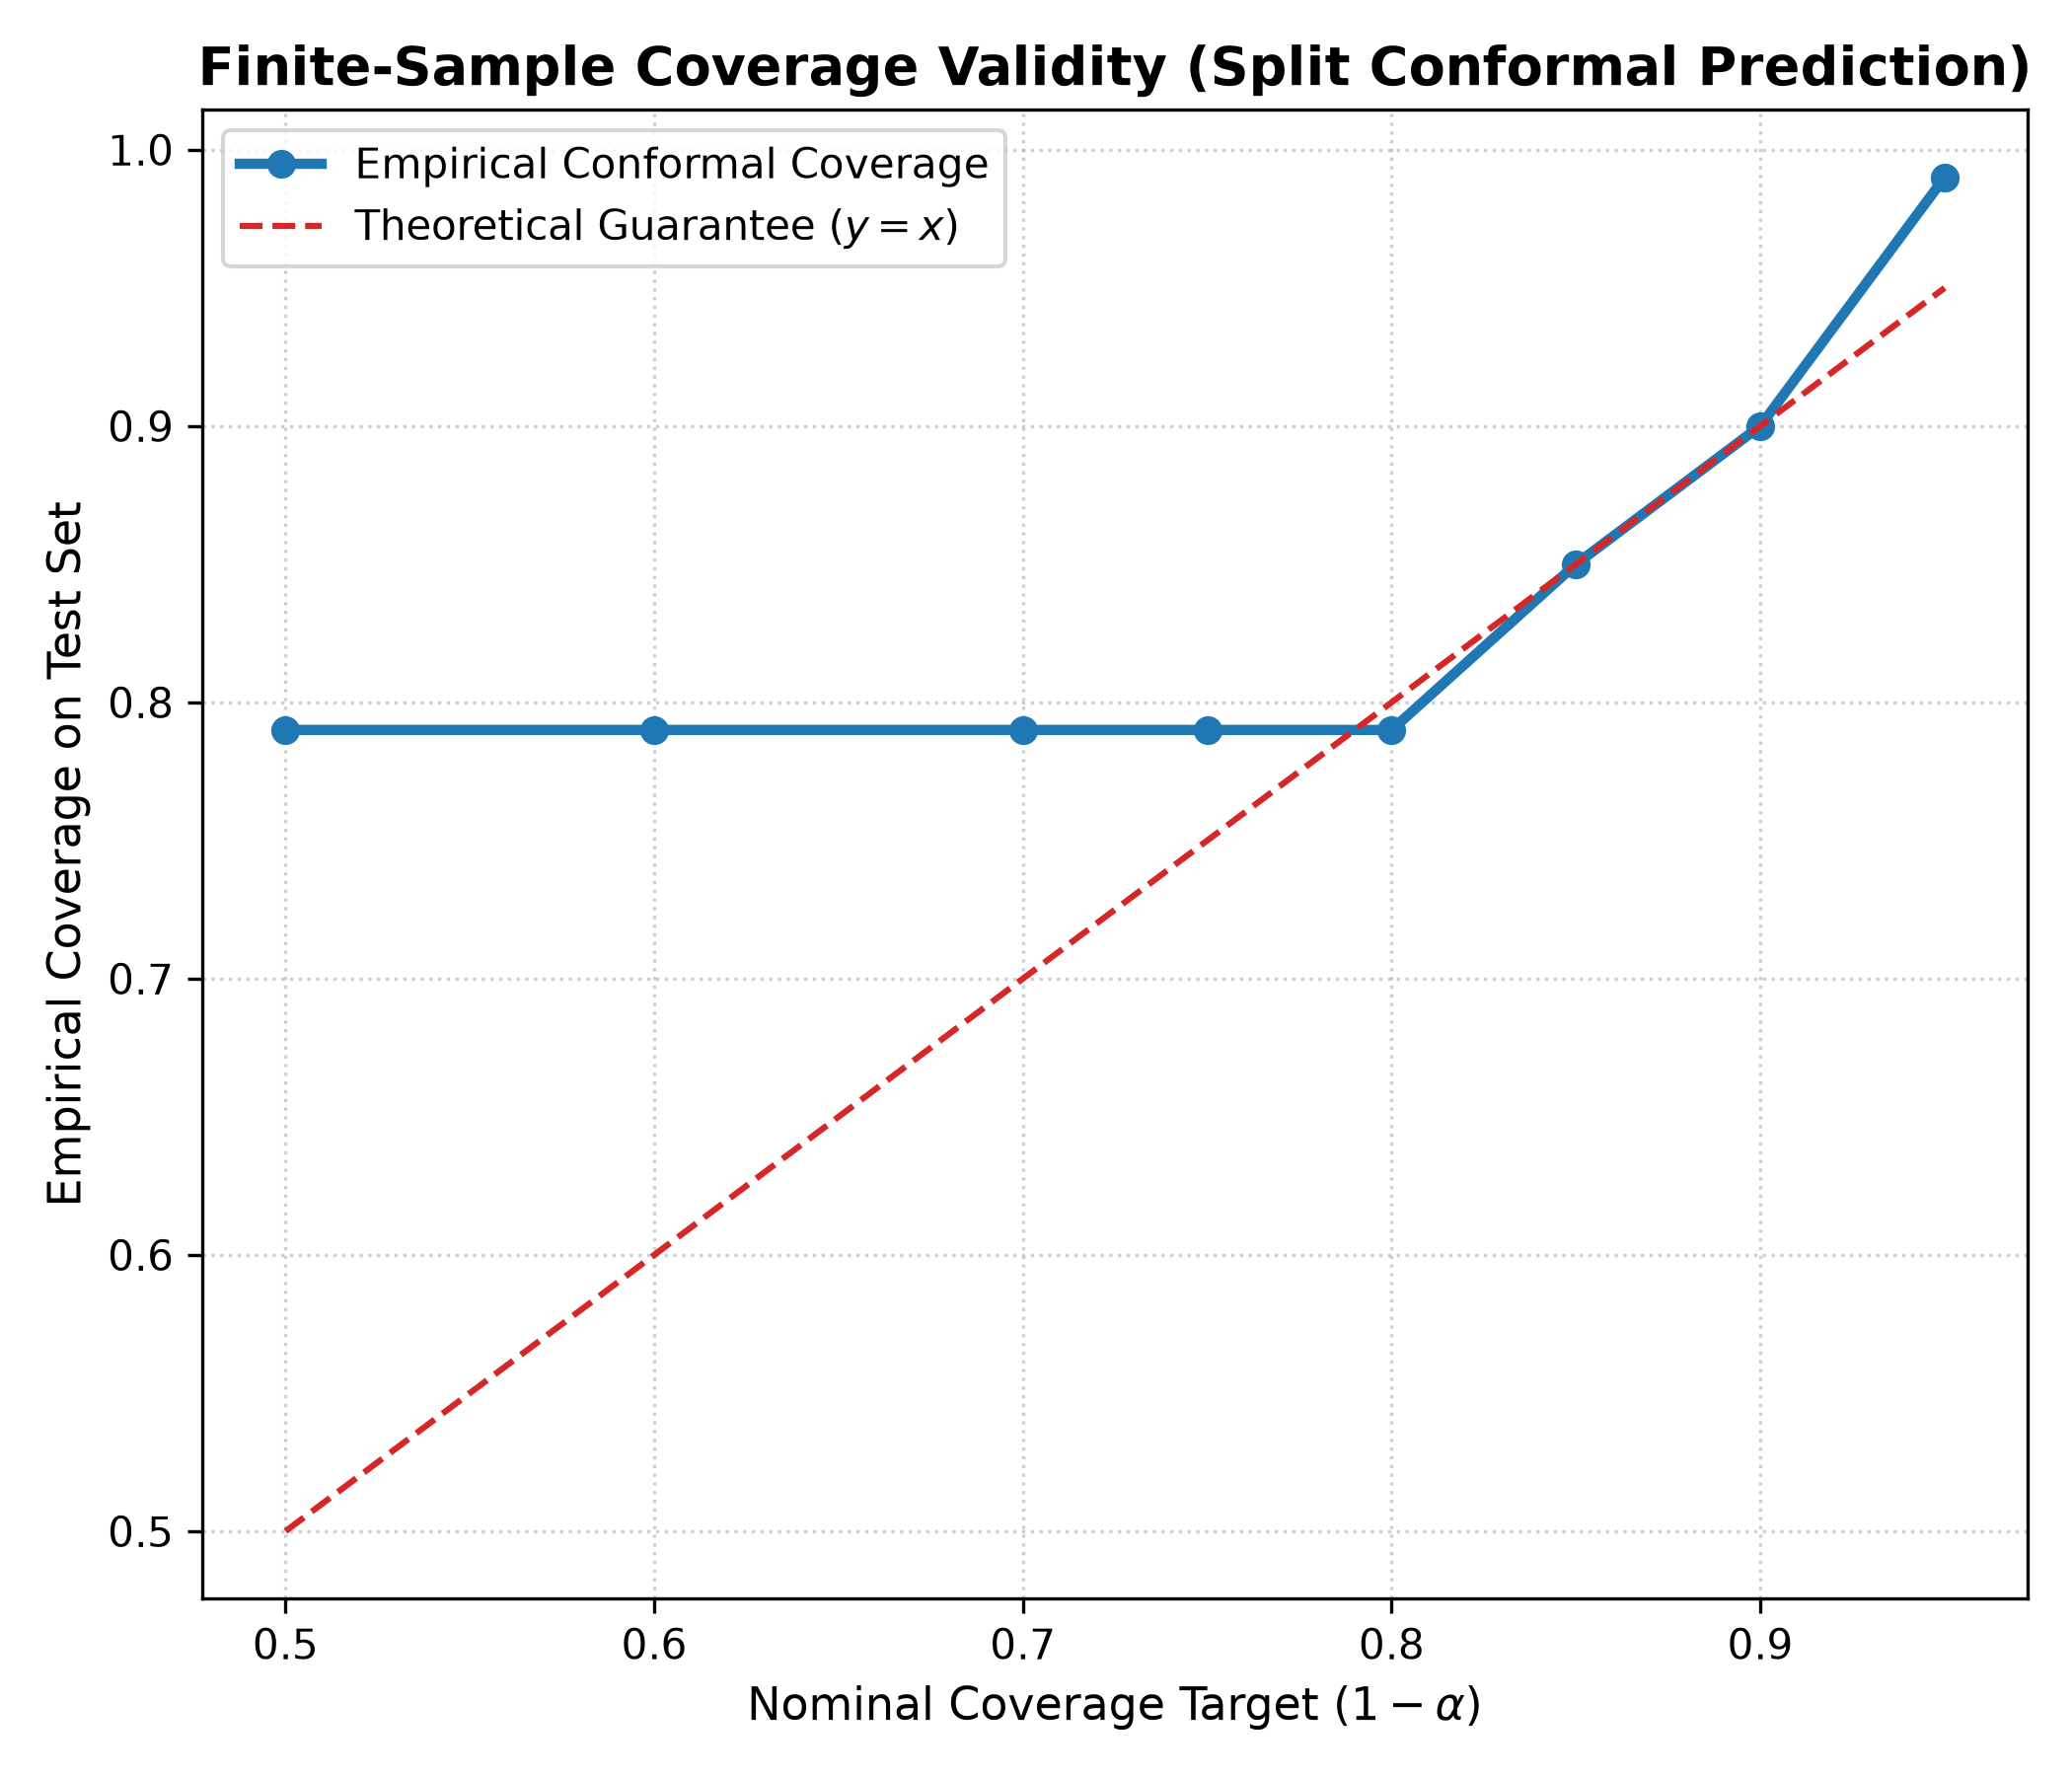
\includegraphics[width=\textwidth]{conformal_coverage_plot.png}
  \caption{Empirical against nominal coverage.}
\end{subfigure}
\hfill
\begin{subfigure}{0.49\textwidth}
  \centering
  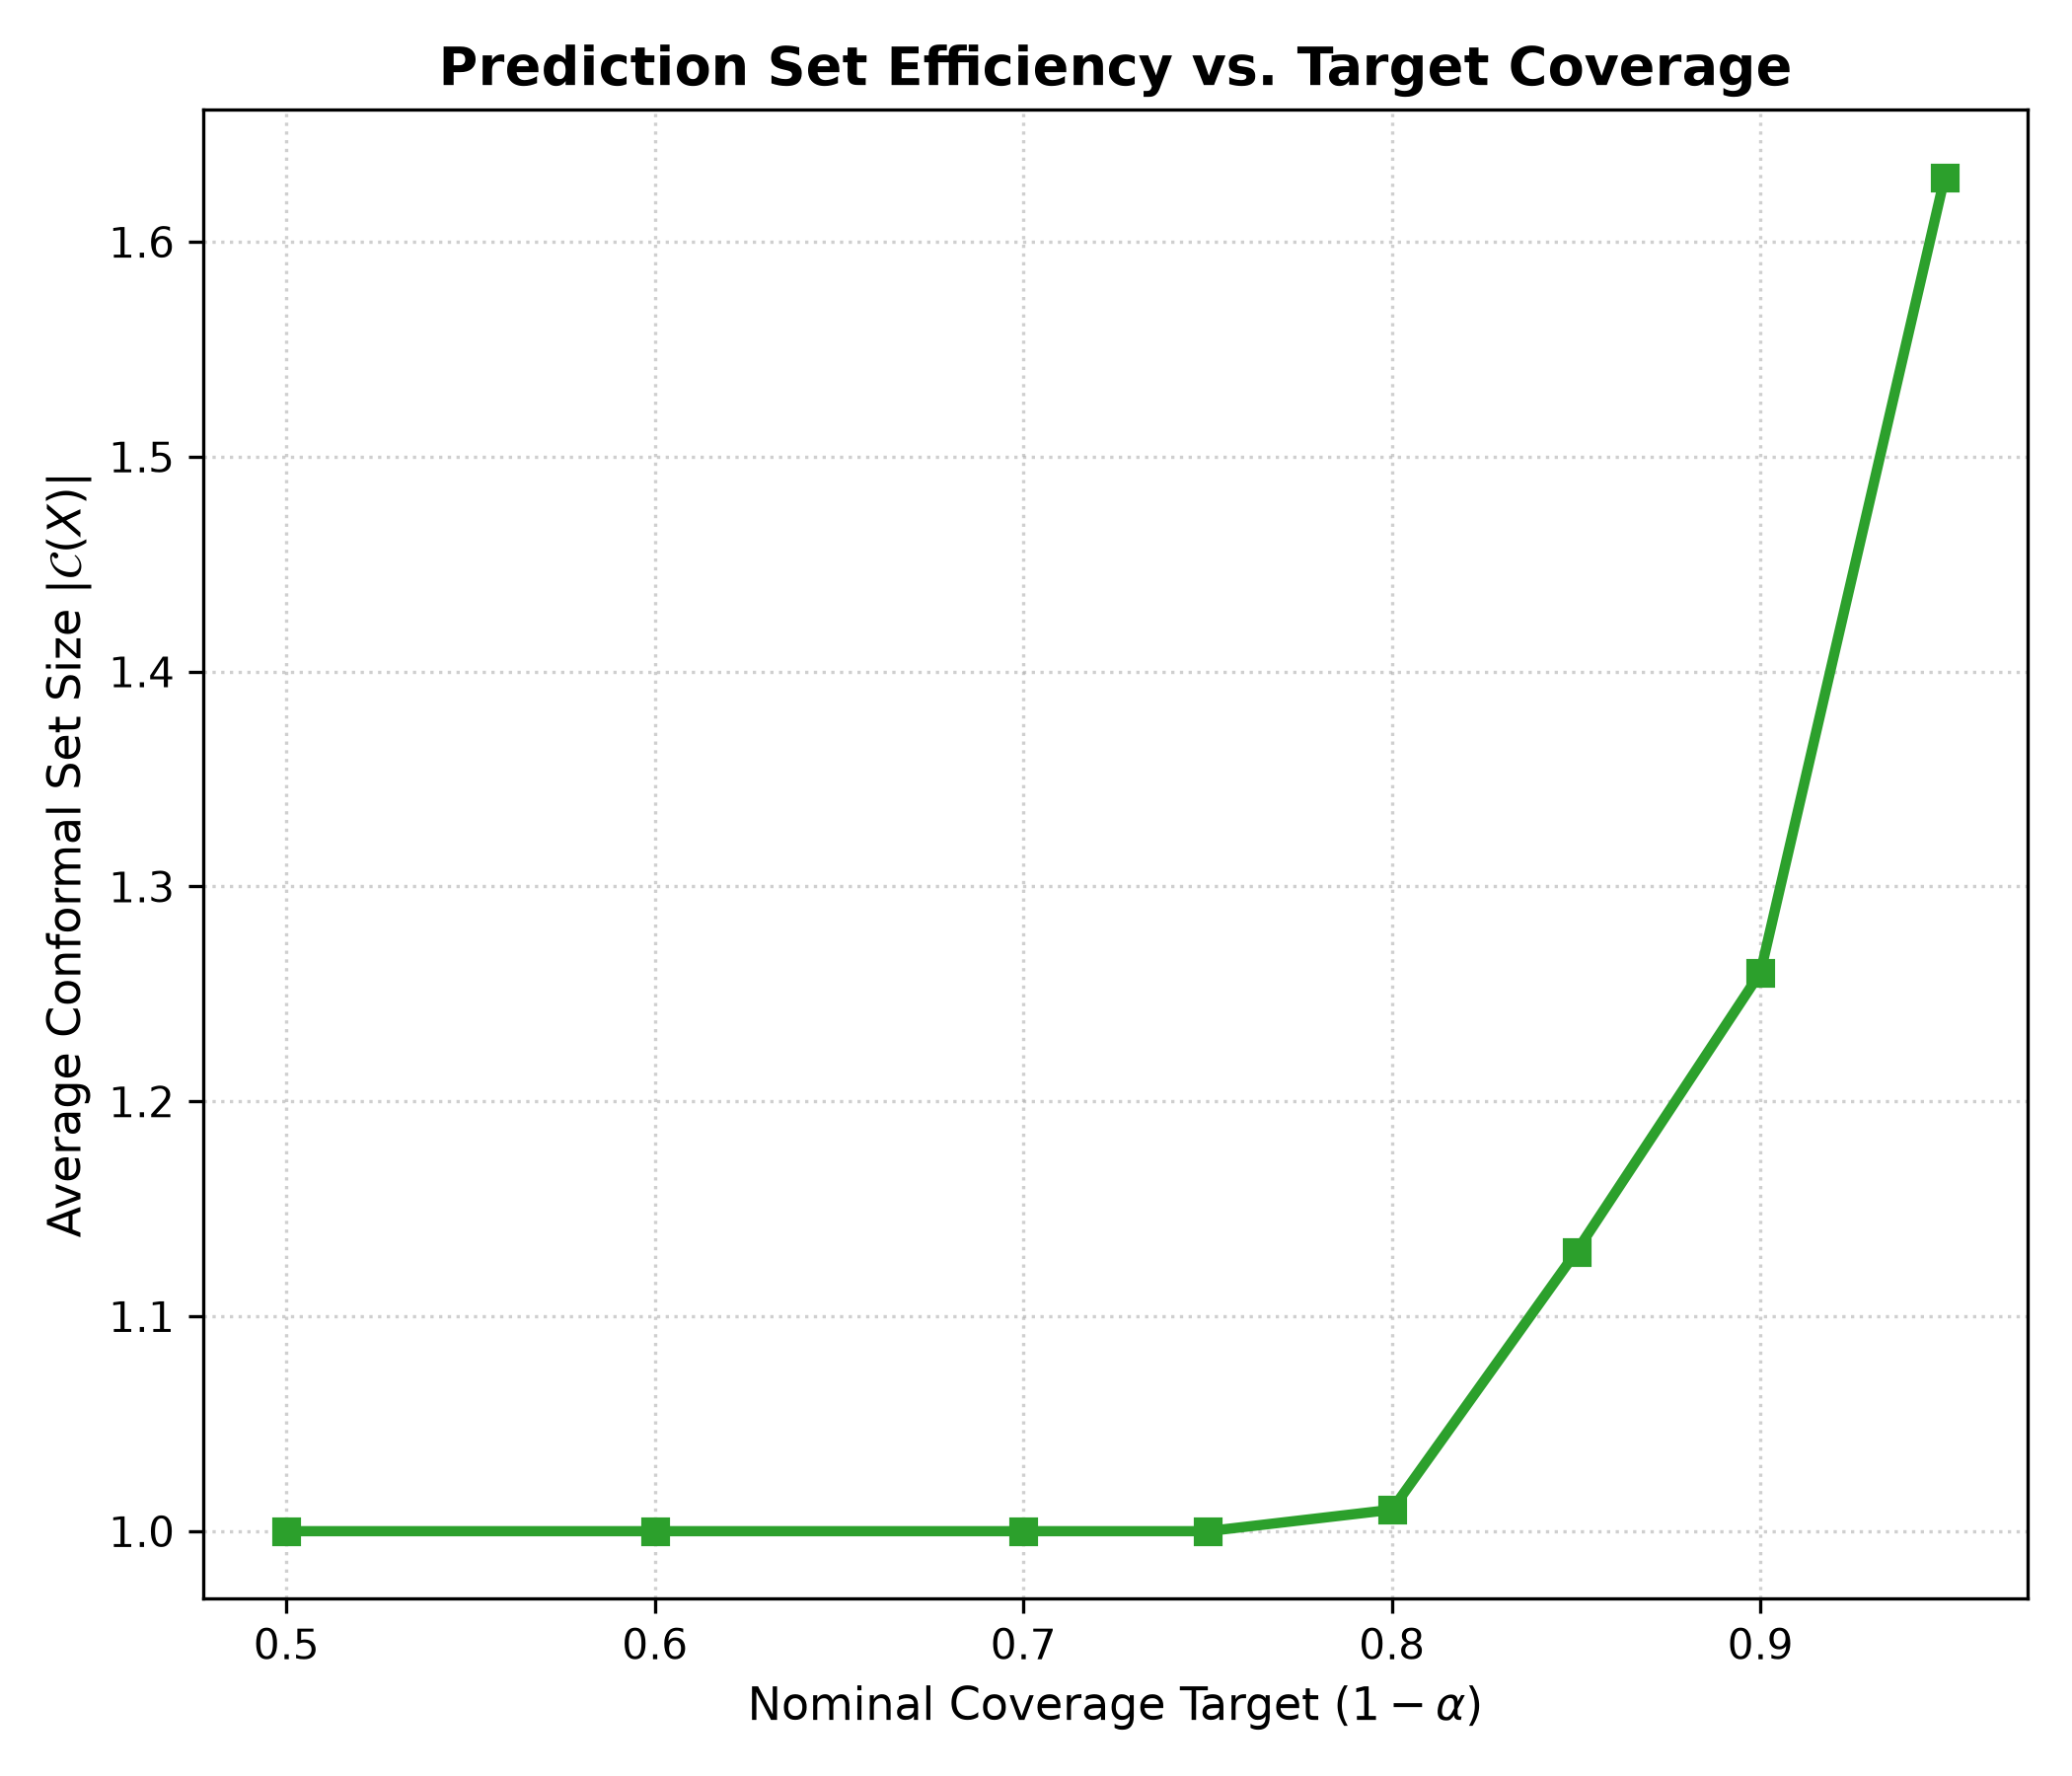
\includegraphics[width=\textwidth]{conformal_set_size_plot.png}
  \caption{Mean prediction-set size.}
\end{subfigure}
\caption{Split conformal prediction on FEVER with gold evidence.}
\label{fig:conformal}
\end{figure}

At the production level $\alpha = 0.10$ the empirical coverage equals the nominal 90\% with only 1.26 labels per set on average, so most claims receive a decisive singleton. For $\alpha \ge 0.20$ the sets are almost always singletons, so coverage cannot fall further and stays at the raw accuracy of the NLI model on gold evidence (79\%).

\subsection{Coverage on retrieved evidence}
\label{sec:coverage-retrieved}

In deployment the NLI probabilities are computed on \emph{retrieved} snippets, which are noisier than FEVER's gold evidence, so the exchangeability assumption of Theorem~\ref{thm:coverage} does not hold. Measuring coverage on the 600 evaluation claims (Table~\ref{tab:coverage-retrieved}, Figure~\ref{fig:coverage-retrieved}) confirms the consequence. To recalibrate without bias, the claims were split into two halves, and each half was tested with the $\hat{q}$ calibrated on the other.

\begin{table}[htbp]
\centering
\caption{Conformal coverage on retrieved evidence (600 claims).}
\label{tab:coverage-retrieved}
\small
\begin{tabularx}{\textwidth}{@{}Xcccc@{}}
\toprule
Threshold & Coverage & Wilson 95\% CI & Mean set size & Accuracy (FEVER / FreshQA) \\
\midrule
Current, $\hat{q} = 0.8985$ (gold-evidence calibration) & 83.2\% & [80.0\%, 85.9\%] & 1.18 & 90.7\% / 82.3\% (measured) \\
Recalibrated on retrieved evidence, $\hat{q} \approx 0.990$--$0.995$ & 90.3\% & [87.7\%, 92.4\%] & 1.80 & 92.3\% / 84.3\% (estimated) \\
\bottomrule
\end{tabularx}
\end{table}

\begin{figure}[htbp]
\centering
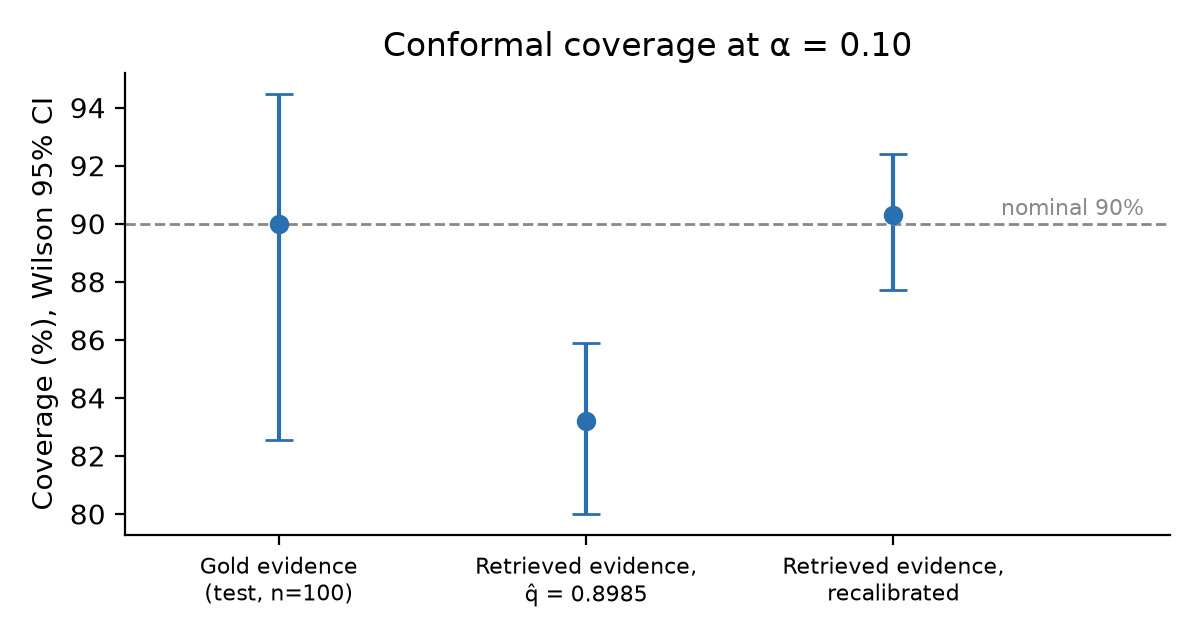
\includegraphics[width=0.7\textwidth]{coverage_retrieved.png}
\caption{Conformal coverage at $\alpha = 0.10$ on gold and retrieved evidence, with Wilson 95\% intervals.}
\label{fig:coverage-retrieved}
\end{figure}

With the current threshold, coverage on live evidence is measurably below the nominal 90\%: the whole interval lies below it, as the exchangeability argument predicts. Recalibrating restores 90.3\% coverage, but only with a threshold that admits any label above about 0.5--1\% probability, so 181 more claims would be escalated. The estimated pooled accuracy would rise from 86.5\% to 88.3\% (530 against 519 correct), but the gain is not significant: the recalibrated verdicts fix 21 claims and break 10 (exact McNemar $p = 0.07$), at the cost of an LLM review for almost a third of all claims. The production threshold is therefore kept, and the conformal set is described as what it is in deployment: a calibrated escalation trigger with 83.2\% measured coverage, not a 90\% guarantee.

\subsection{Class-conditional coverage and alternative scores}
\label{sec:conformal-variants}

Two questions remain: whether the shortfall falls equally on false and true claims, and whether a different conformal procedure (Section~\ref{sec:scores}) would do better. Four procedures were compared at $\alpha = 0.10$: the production layer (LAC), Mondrian LAC, non-randomised APS, and randomised APS as a reference (one uniform draw per claim, fixed seed). Each was calibrated on the 100 production calibration claims and evaluated in three settings: on the other 100 gold-evidence claims; on the 600 benchmark claims with the gold-evidence quantiles, as deployed; and on the 600 claims recalibrated by the same two-fold cross-fitting as in Table~\ref{tab:coverage-retrieved}. For the benchmark claims, the routing rule~\eqref{eq:escalate} was applied to each procedure's sets. A claim keeps its verdict unless its route changes. A claim that no longer goes to the LLM takes its NLI verdict, and a newly escalated claim takes the LLM verdict on its saved evidence from Section~\ref{sec:llm-baseline}, so no new LLM call is needed. As a check, the production layer reproduces the routing of the run exactly (98 escalations, no verdict changed).

\begin{table}[H]
\centering
\caption{Conformal procedures on gold evidence (calibrated on 100 claims, tested on 100: 45 false, 55 true).}
\label{tab:conformal-gold}
\small
\begin{tabular}{@{}lcccc@{}}
\toprule
Procedure & Coverage (95\% CI) & False claims & True claims & Mean set size \\
\midrule
LAC (production) & 90.0\% [82.6, 94.5] & 95.6\% & 85.5\% & 1.26 \\
Mondrian LAC & 92.0\% [85.0, 95.9] & 84.4\% & 98.2\% & 1.26 \\
APS & 95.0\% [88.8, 97.8] & 95.6\% & 94.5\% & 1.76 \\
Randomised APS & 92.0\% [85.0, 95.9] & 95.6\% & 89.1\% & 1.41 \\
\bottomrule
\end{tabular}
\end{table}

\begin{table}[H]
\centering
\caption{Conformal procedures on retrieved evidence (600 claims: 297 false, 303 true), with the number of claims escalated, the estimated pooled accuracy, and the exact McNemar test against the pipeline as run ($b$: right only as run; $c$: right only with the procedure).}
\label{tab:conformal-variants}
\resizebox{\textwidth}{!}{%
\begin{tabular}{@{}llcccccccc@{}}
\toprule
Quantiles & Procedure & Coverage (Wilson 95\% CI) & False claims & True claims & Set size & Escalated & Accuracy & $b$ / $c$ & $p$ \\
\midrule
Gold-evidence & LAC (production) & 83.2\% [80.0, 85.9] & 84.5\% & 81.8\% & 1.18 & 98 & 86.5\% & -- & -- \\
(as deployed) & Mondrian LAC & 83.3\% [80.1, 86.1] & 79.8\% & 86.8\% & 1.19 & 125 & 87.2\% & 1 / 5 & 0.22 \\
 & APS & 86.7\% [83.7, 89.2] & 87.5\% & 85.8\% & 1.83 & 483 & 88.8\% & 14 / 28 & 0.044 \\
 & Randomised APS & 85.0\% [81.9, 87.6] & 86.2\% & 83.8\% & 1.35 & 184 & 86.8\% & 7 / 9 & 0.80 \\
\midrule
Recalibrated & LAC & 90.3\% [87.7, 92.4] & 92.6\% & 88.1\% & 1.80 & 339 & 88.3\% & 10 / 21 & 0.071 \\
(cross-fitted) & Mondrian LAC & 90.3\% [87.7, 92.4] & 89.6\% & 91.1\% & 1.82 & 350 & 88.0\% & 12 / 21 & 0.16 \\
 & APS & 90.2\% [87.5, 92.3] & 89.9\% & 90.4\% & 2.33 & 600 & 88.2\% & 18 / 28 & 0.18 \\
 & Randomised APS & 90.2\% [87.5, 92.3] & 92.3\% & 88.1\% & 1.90 & 388 & 88.0\% & 15 / 24 & 0.20 \\
\bottomrule
\end{tabular}}
\end{table}

\begin{figure}[H]
\centering
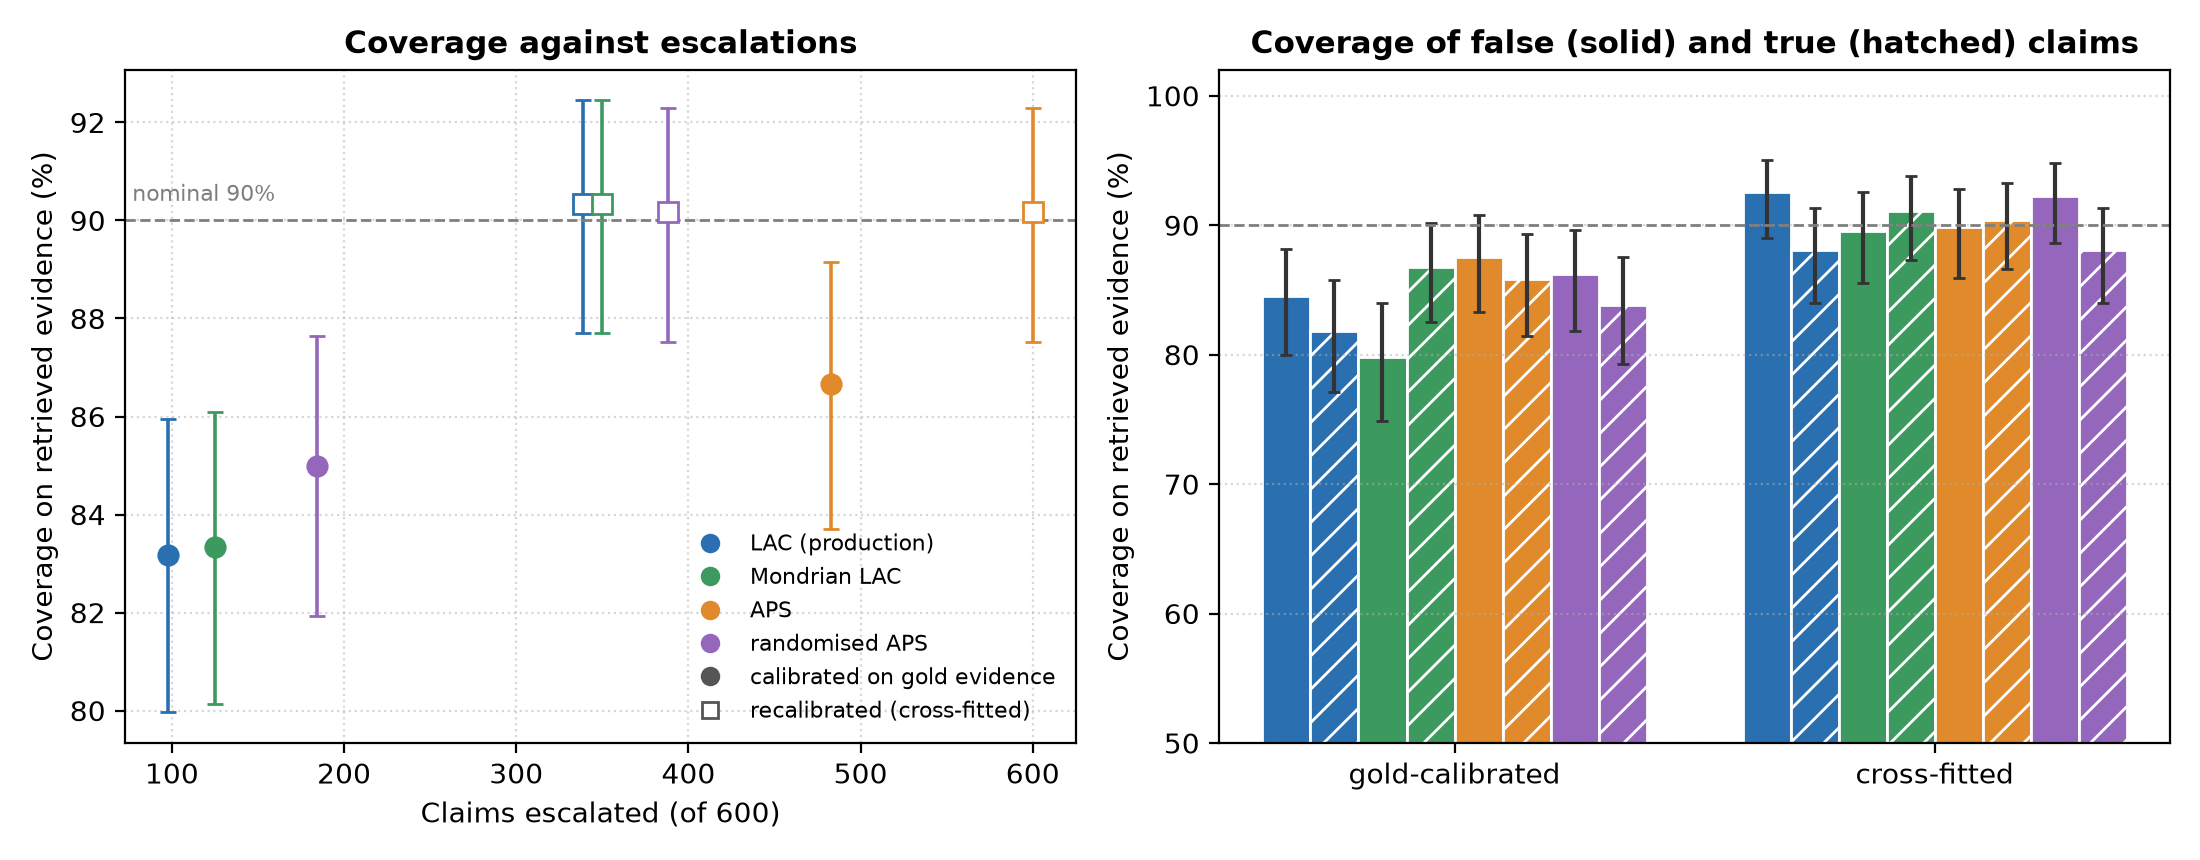
\includegraphics[width=\textwidth]{conformal_variants.png}
\caption{Conformal procedures on retrieved evidence. Left: coverage against the number of claims escalated, with gold-evidence quantiles (filled) and cross-fitted recalibration (open). Right: coverage of false (solid) and true (hatched) claims, with Wilson 95\% intervals.}
\label{fig:conformal-variants}
\end{figure}

The results (Tables~\ref{tab:conformal-gold} and~\ref{tab:conformal-variants}, Figure~\ref{fig:conformal-variants}) answer both questions:
\begin{itemize}[itemsep=0.3em]
  \item \textbf{The shortfall is shared by both classes.} On retrieved evidence the production layer covers 84.5\% of false claims and 81.8\% of true claims, and the two intervals overlap. Hallucinations are not disproportionately missed. On gold evidence the imbalance runs the other way (95.6\% against 85.5\%), because false FEVER claims are refuted confidently by their gold evidence.
  \item \textbf{Mondrian balances the classes, as Theorem~\ref{thm:mondrian} predicts, but does not repair the shift.} Recalibrated, it brings both classes close to 90\% (89.6\% and 91.1\%, against 92.6\% and 88.1\% for LAC) at almost the same cost (350 escalations against 339). With the gold-evidence quantiles its overall coverage stays at 83.3\%. On gold evidence its false-claim coverage of 84.4\% is below 90\%, but with 45 test claims and about 50 calibration claims per class this lies within the expected variation of one calibration.
  \item \textbf{Non-randomised APS degenerates as Remark~\ref{rem:aps} predicts.} Its quantile is 0.9998 on gold evidence and 1.0000 when recalibrated, so it escalates 483 and 600 claims. Its higher coverage and accuracy come only from sending almost every claim to the LLM; recalibrated, it reproduces the LLM-only baseline of Section~\ref{sec:llm-baseline} exactly.
  \item \textbf{Randomised APS is less efficient than LAC.} It reaches 90\% coverage only with 388 escalations, against 339 for LAC, with no gain in accuracy.
\end{itemize}

None of the accuracy differences in Table~\ref{tab:conformal-variants} survives a Holm correction over its seven comparisons; the smallest $p$, 0.044, becomes 0.31. LAC is the most efficient of the four procedures, and no choice of score closes the gap between 83\% and 90\% without escalating hundreds more claims. The shortfall comes from the difference between gold and retrieved evidence, not from the procedure, which is why the production layer is kept and reported as a calibrated escalation trigger.

\section{Calibration of the NLI Probabilities}

Calibration was evaluated on the 560 benchmark claims whose final NLI verdict is \Sup{} or \Con. The temperature $T$ was cross-fitted: each set was scored with the $T$ fitted on the other sets (the fitted values range from 2.43 to 2.56; on all claims $T = 2.48$). A paired bootstrap with 10{,}000 resamples~\citep{efron1993bootstrap} gives 95\% intervals for each change (Table~\ref{tab:calibration}).

\begin{table}[htbp]
\centering
\caption{Calibration before and after temperature scaling (560 claims).}
\label{tab:calibration}
\begin{tabular}{@{}lccc@{}}
\toprule
Metric & Raw & Temperature-scaled & Change (95\% bootstrap interval) \\
\midrule
NLL & 0.898 & 0.585 & $-0.313$ [$-0.423$, $-0.207$] \\
Brier score & 0.296 & 0.286 & $-0.010$ [$-0.028$, $+0.006$] \\
ECE & 11.4\% & 5.7\% & $-5.7$ points [$-8.9$, $-0.4$] \\
Mean confidence & 95.7\% & 79.6\% & -- \\
Accuracy & 84.6\% & 84.6\% & unchanged \\
\bottomrule
\end{tabular}
\end{table}

\begin{figure}[htbp]
\centering
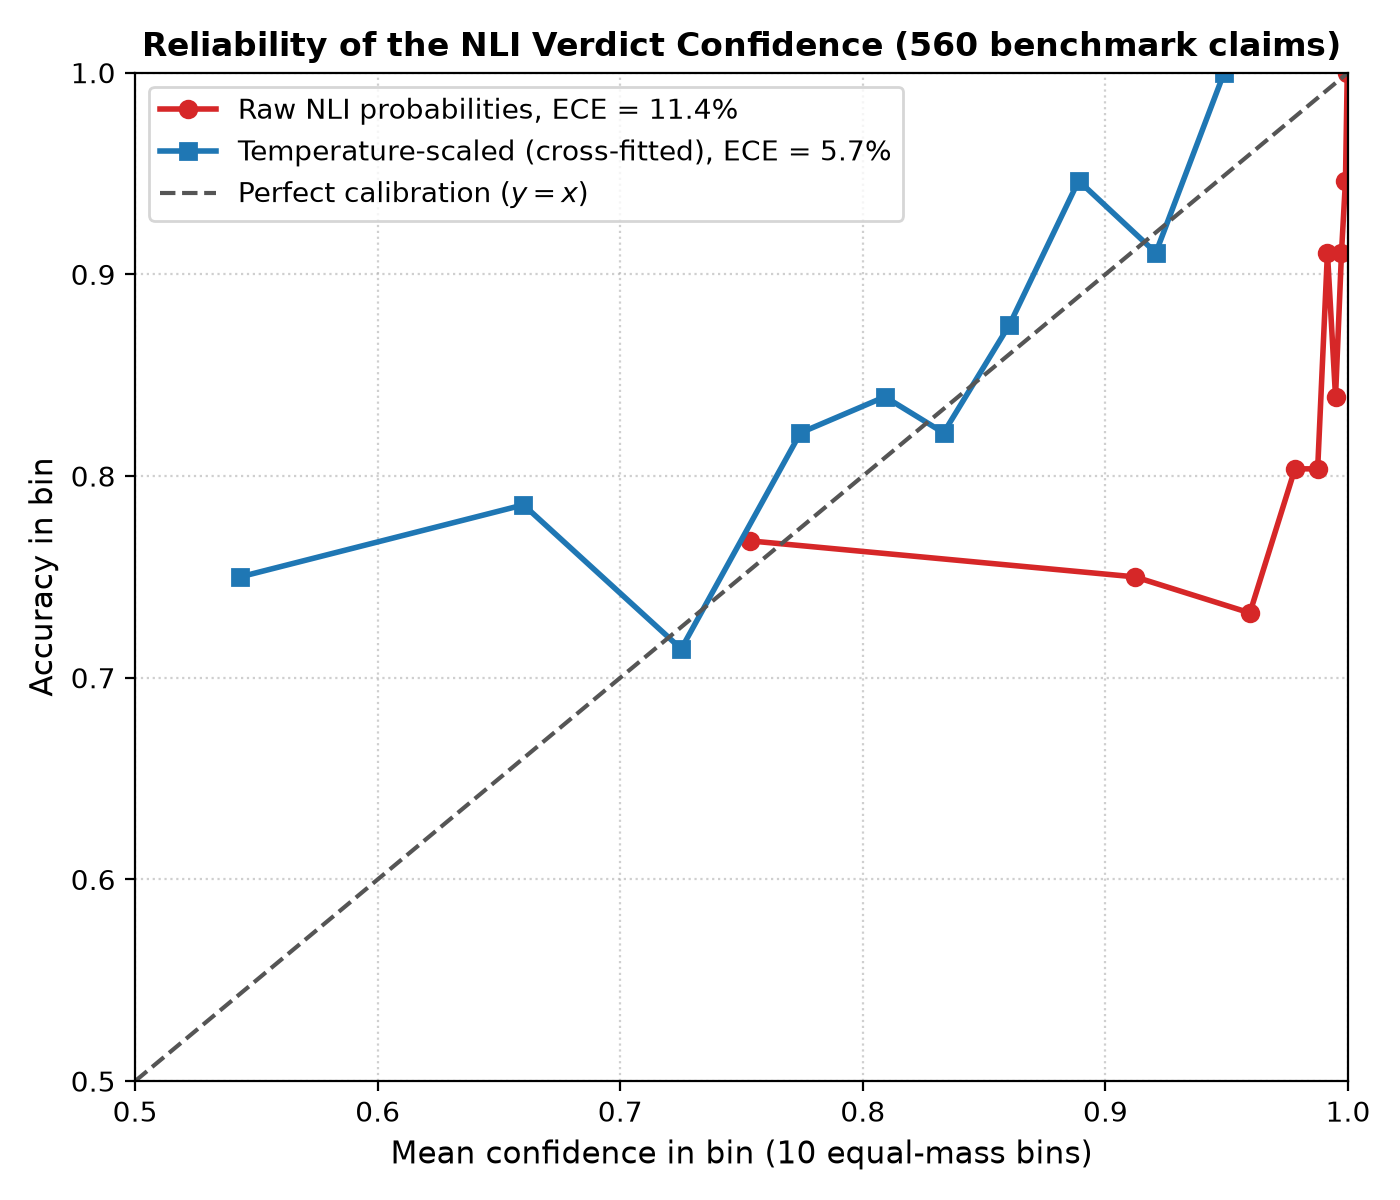
\includegraphics[width=0.75\textwidth]{calibration_reliability.png}
\caption{Reliability diagram of the NLI confidence before and after temperature scaling (ten bins of 56 claims).}
\label{fig:reliability}
\end{figure}

The raw confidences crowd above 0.95 while accuracy ranges from 73\% to 100\% across bins. After scaling, the stated confidence tracks accuracy in most bins (Figure~\ref{fig:reliability}). The NLL improvement is clearly significant, because it comes from the confident mistakes that scaling softens, and so is the halving of the ECE. The Brier improvement is not: the Brier score also rewards ranking right verdicts above wrong ones, which a single temperature hardly changes. Indeed the raw confidence separates right from wrong verdicts with an AUROC of 0.672 and the scaled confidence with 0.673. For the \emph{Bones} example, the logits $(4.084, -0.974, -3.995)$ become $(1.646, -0.393, -1.610)$, and the confidence in \Con{} falls from 0.993 to 0.856. Decisions keep the raw scale, because the thresholds and the conformal quantile were set and measured on it; the calibrated confidence is reported alongside.

A two-parameter Platt scaling, cross-fitted in the same way, reaches a top-label ECE of 5.5\% against 5.7\%, a difference within noise; temperature scaling is kept because it has one parameter and yields a full probability vector.

\section{Selective Prediction}
\label{sec:selective-results}

The pipeline already abstains on 4 FEVER and 15 FreshQA claims. Section~\ref{sec:selective} asks a further question: if the detector were allowed to abstain on more claims, would its NLI confidence choose the right ones? The answered claims were ranked by the NLI probability of their final verdict, and the detector abstained on the least confident first (Figure~\ref{fig:risk-coverage}, Table~\ref{tab:selective}). The AURC interval is a percentile bootstrap over the answered claims (1{,}000 resamples).

\begin{figure}[H]
\centering
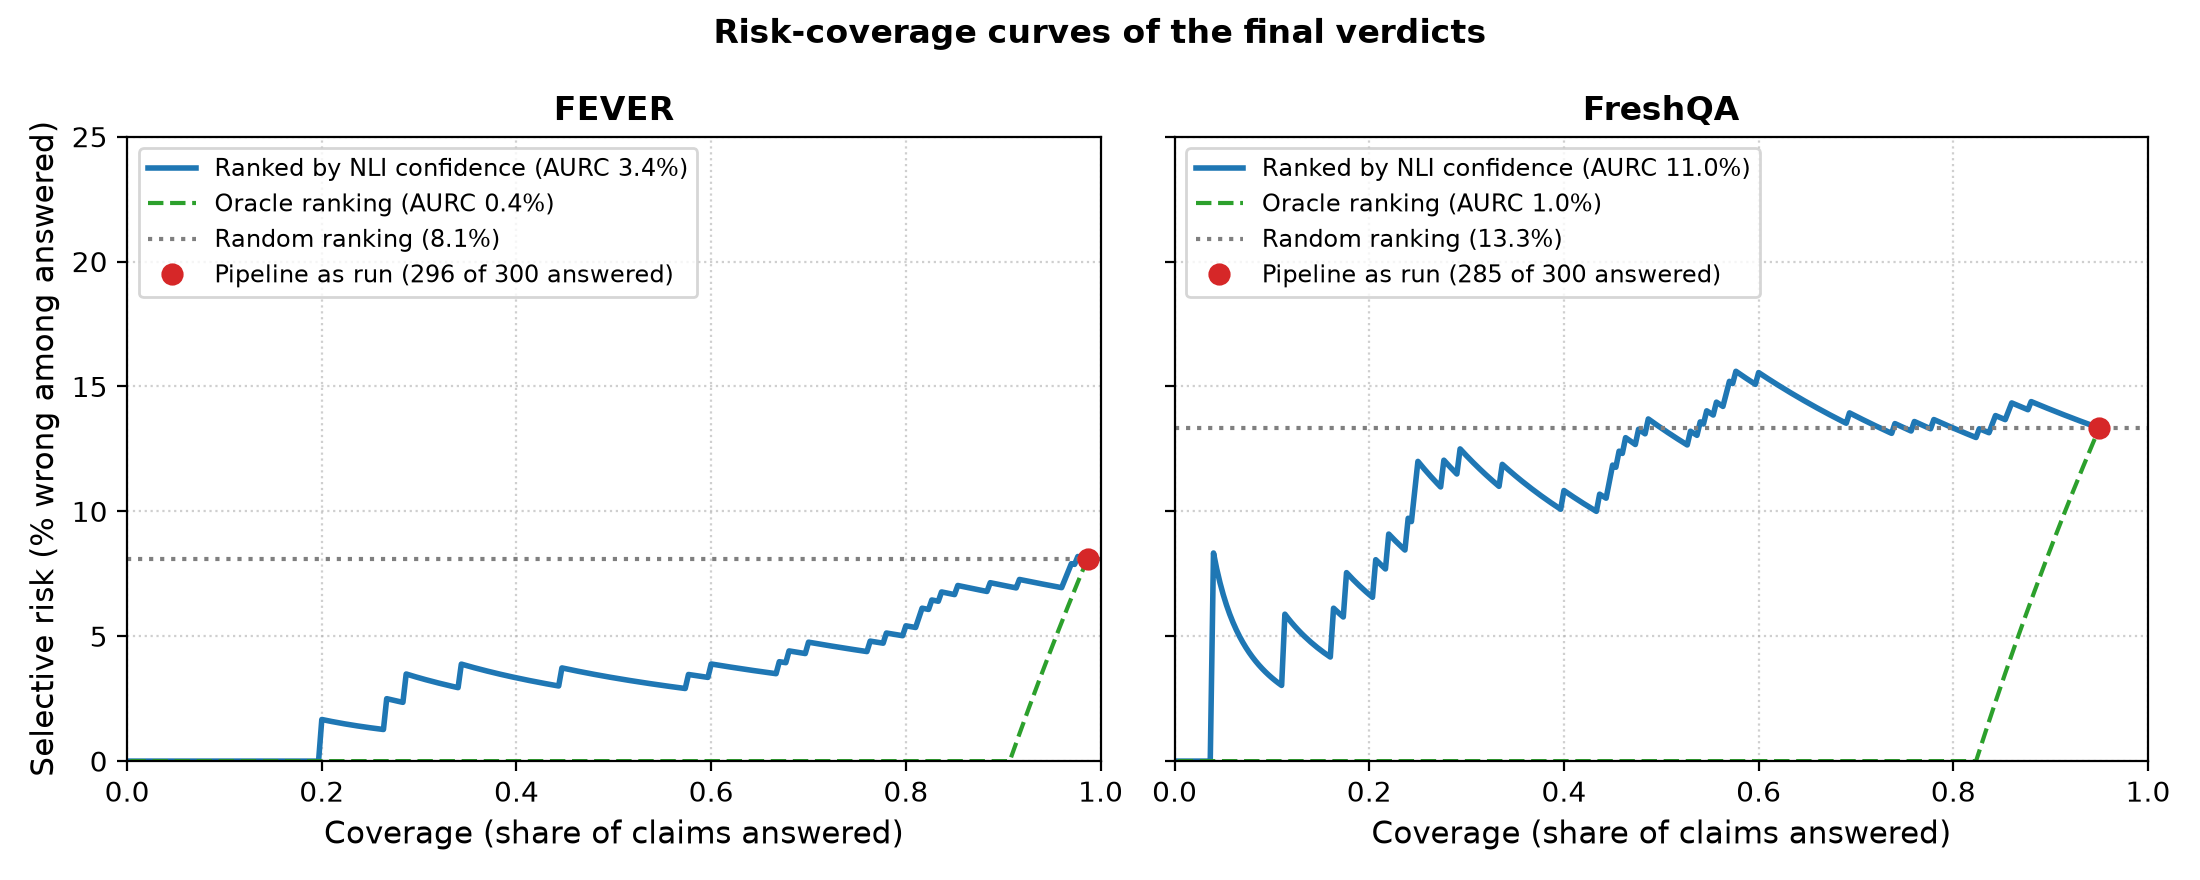
\includegraphics[width=\textwidth]{risk_coverage.png}
\caption{Risk--coverage curves of the final verdicts, ranked by the NLI probability of the verdict, against the oracle and random rankings of Proposition~\ref{prop:aurc}. The red point is the pipeline as run.}
\label{fig:risk-coverage}
\end{figure}

\begin{table}[H]
\centering
\caption{Selective prediction. Selective risk is the error rate among answered claims.}
\label{tab:selective}
\resizebox{\textwidth}{!}{%
\begin{tabular}{@{}lcccccc@{}}
\toprule
Benchmark & Answered & Risk as run & AURC (95\% CI) & Oracle & Random & Risk at 80\% / 90\% coverage \\
\midrule
FEVER & 296 / 300 & 8.1\% & 3.4\% [1.5, 5.5] & 0.35\% & 8.1\% & 5.4\% / 7.0\% \\
FreshQA & 285 / 300 & 13.3\% & 11.0\% [6.8, 16.1] & 0.95\% & 13.3\% & 13.3\% / 14.1\% \\
\bottomrule
\end{tabular}}
\end{table}

On FEVER the confidence is informative. Its AURC is less than half the random value, and abstaining on the least confident fifth of the claims lowers the error rate among the rest from 8.1\% to 5.4\%. On FreshQA the confidence helps only among the most confident quarter of the claims; at 80\% and 90\% coverage the selective risk equals the overall error rate, so abstaining by confidence would not help. The reason lies in FreshQA's errors (Section~\ref{sec:errors}): most are confident NLI fast-path errors on time-dependent claims and false premises, or claims whose gold label is out of date, and the NLI confidence cannot identify either kind. Both curves stay far above the oracle. This agrees with the moderate AUROC of the confidence (0.67, Section~\ref{sec:calibration}) and confirms that better abstention and routing need signals beyond the NLI confidence.

\section{Summary of Hypothesis Tests}
\label{sec:test-summary}

Table~\ref{tab:tests} collects the eight hypothesis tests reported, with their Holm and Benjamini--Hochberg adjusted $p$-values (Section~\ref{sec:multiple}).

\begin{table}[htbp]
\centering
\caption{All hypothesis tests with multiple-comparison corrections. Bold marks an adjusted $p < 0.05$.}
\label{tab:tests}
\small
\begin{tabularx}{\textwidth}{@{}Xllll@{}}
\toprule
Comparison & Test & $p$ & Holm & BH \\
\midrule
LLM arbiter vs NLI verdict, both benchmarks (60 fixed, 15 broken) & exact McNemar & $1.6 \times 10^{-7}$ & $\mathbf{1.3 \times 10^{-6}}$ & $\mathbf{1.3 \times 10^{-6}}$ \\
LLM arbiter, FreshQA (42 fixed, 8 broken) & exact McNemar & $1.2 \times 10^{-6}$ & $\mathbf{8.1 \times 10^{-6}}$ & $\mathbf{4.7 \times 10^{-6}}$ \\
Corroboration rule, $m = 2$ vs $m = 1$ (21 vs 5) & exact McNemar & 0.002 & \textbf{0.015} & \textbf{0.006} \\
FEVER vs FreshQA accuracy (90.7\% vs 82.3\%) & two-proportion $z$ & 0.003 & \textbf{0.015} & \textbf{0.006} \\
LLM arbiter, FEVER (18 fixed, 7 broken) & exact McNemar & 0.043 & 0.17 & 0.069 \\
FEVER, the three runs (95, 87, 90 of 100) & $\chi^2_2$ & 0.15 & 0.44 & 0.19 \\
FreshQA, the three runs (82, 85, 80 of 100) & $\chi^2_2$ & 0.65 & 1 & 0.74 \\
Corroboration rule, $m = 2$ vs $m = 3$ (2 vs 2) & exact McNemar & 1 & 1 & 1 \\
\bottomrule
\end{tabularx}
\end{table}

The ablation comparisons of Section~\ref{sec:ablation} form a separate family with their own Holm correction and are not included here. Four findings survive both corrections: the arbiter improves on the NLI verdict (pooled, and on FreshQA alone), $m = 2$ beats $m = 1$, and FreshQA is harder than FEVER. The arbiter's effect on FEVER alone is significant only before correction; the runs of each benchmark are mutually consistent; and $m = 2$ and $m = 3$ cannot be told apart.

\paragraph{Power.} Non-significant results must be read against the power of the test. With 300 claims per benchmark, a true difference of 5 points between benchmarks (around 86.5\% accuracy) would be detected with only 43\% power (44\% in simulation), 7.5 points with 77\% and 10 points with 95\%; 80\% power for a 5-point difference would need 733 claims per benchmark. At the observed difference of 8.3 points, 263 claims per benchmark give 80\% power, so the present 300 suffice. For the arbiter on FEVER ($\psi = 0.35$, $\delta = 0.15$) about 113 arbitrated claims, roughly 480 FEVER claims, would be needed, against 71 now. The non-significant FEVER arbiter result is therefore expected at this sample size and does not show that the arbiter has no effect there.

\section{Error Analysis}
\label{sec:errors}

\subsection{FEVER}

The 28 FEVER errors are 9 false accusations, 15 missed hallucinations and 4 abstentions. By the stage that produced them:
\begin{itemize}[itemsep=0.3em]
  \item \textbf{NLI fast-path errors (17).} Settled without LLM review. True claims were contradicted by several agreeing snippets that describe a related but different fact (e.g.\ \emph{``Taran Killam is an American writer''}, contradicted by snippets describing him as an actor and comedian), or because the query retrieved the wrong sense of an ambiguous name (\emph{``Tool is a band''} retrieved the article on tools as implements). False claims were supported by a decisive snippet about a closely related fact (\emph{``Saturn is the second-largest moon in the Solar System''}, supported by a sentence stating this of Titan, Saturn's largest moon), or differing from the evidence in a single number, title or role.
  \item \textbf{Arbiter errors (7).} Mostly over-generous inference, such as accepting \emph{``Heavy metal music was developed in Europe''} from evidence that it developed ``largely in the United Kingdom and United States'', or reading a present-tense claim as contradicted by evidence of a past state.
  \item \textbf{Abstentions (4).} The evidence covered the topic but not the specific fact, and the arbiter, finding no statement either way, abstained.
\end{itemize}

\subsection{FreshQA}

\begin{table}[htbp]
\centering
\caption{FreshQA accuracy by fact type.}
\label{tab:facttype}
\begin{tabular}{@{}lcccc@{}}
\toprule
Fact type & Claims & Correct & Wrong & Accuracy \\
\midrule
never-changing & 155 & 130 & 25 & 83.9\% \\
slow-changing & 145 & 117 & 28 & 80.7\% \\
\bottomrule
\end{tabular}
\end{table}

The 53 FreshQA errors fall into four groups:
\begin{itemize}[itemsep=0.3em]
  \item \textbf{NLI fast-path errors (24).} Negations, claims about the present matched to past evidence (the NLI model ignores words such as \emph{``currently''}), false premises accepted from related evidence (\emph{``Hikaru Nakamura became the World Chess Champion''}, supported by snippets on his Fischer Random world title), and web pages that themselves assert a false claim.
  \item \textbf{Abstentions (15).} In all but one, the evidence covered the topic but not the specific number, date or ranking the claim asserts. In one case the claim-echo filter removed the only snippets stating the fact, because a genuine paraphrase of a short claim reached the 80\% overlap threshold.
  \item \textbf{Gold labels contradicted by current evidence (11).} The evidence retrieved in 2026 states a different value from the dated gold answer (for example, a later record time or a changed station count). In these cases the detector followed the evidence; even slow-changing labels drift out of date.
  \item \textbf{Arbiter errors (3).} Including one case in which the arbiter counted an item from a different, similarly named list.
\end{itemize}

Across both benchmarks, 41 of the 81 errors are NLI fast-path errors and 19 are abstentions, which identifies the two main levers for improvement: routing the claim types on which NLI is systematically weak (negations, time-dependent claims) to the arbiter, and better retrieval of specific numeric facts.
